\section{Integration and Accumulation of Change}
The accumulation of change is the net change of a quantity. This is not the same as simply the quantity. The accumulation of change takes into consideration time, and thus is the quantity over a specified time period. There may be a change in quantity before or after the specified time period, but that is not considered.

\subsection{Riemann Sums}
The Riemann sum is a method used to approximate the area under a curve. It splits up the area into several rectangles of equal width, whose heights match up with the function. The sum of the area of the rectangles would provide an approximation of the area.

The accuracy of the approximation can be improved by increasing the number of rectangles. This is done by decreasing $\Delta x$, the width of each rectangle.

\subsubsection{Types of Riemann Sums}
There are four main types of Riemann sums. Depending on the type of Riemann sum used, there may be either an over or under approximation of the actual area under the curve.
\begin{itemize}
	\item \textbf{Left Riemann Sum:} line up the left side of the rectangle with the curve of the function.
	\begin{figure}[H]
		\centering
		\frame{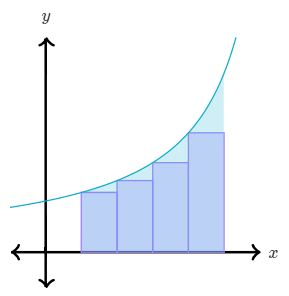
\includegraphics[width=0.4\textwidth]{images/fig9.JPG}}
		\caption{Left Riemann Sum.}
	\end{figure}

	\item \textbf{Right Riemann Sum:} line up the right side of the rectangle with the curve of the function.
	\begin{figure}[H]
		\centering
		\frame{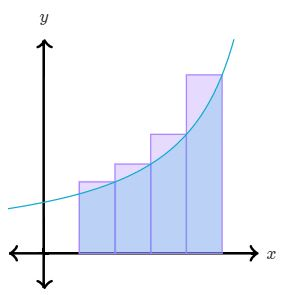
\includegraphics[width=0.4\textwidth]{images/fig10.JPG}}
		\caption{Right Riemann Sum.}
	\end{figure}

	\item \textbf{Midpoint Riemann Sum:} line up the middle of the rectangle with the curve of the function.
	\begin{figure}[H]
		\centering
		\frame{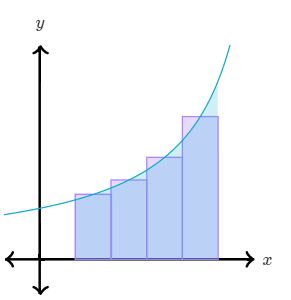
\includegraphics[width=0.4\textwidth]{images/fig11.JPG}}
		\caption{Midpoint Riemann Sum.}
	\end{figure}

	\item \textbf{Trapezoidal Sum:} uses trapezoids of equal height instead of rectangles to provide a better approximation of the area under the curve. The two bases of the trapezoid touch the curve of the function.
	\begin{figure}[H]
		\centering
		\frame{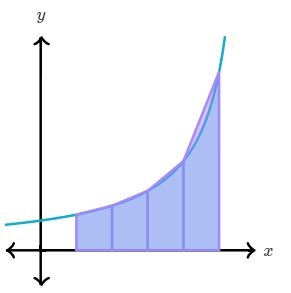
\includegraphics[width=0.4\textwidth]{images/fig12.JPG}}
		\caption{Trapezoidal Sum.}
	\end{figure}
\end{itemize}

\subsubsection{Reimann Sum in Summation Notation}
We want to approximate a function $f(x)$ using a Riemann sum over the interval $[a, b]$ with $n$ rectangles of equal width. We can define the width of each rectangle as ${\Delta x = \frac{b - a}{n}}$.

With \textit{left} Riemann sums, the rectangles can be labelled $i = 0$ through $i = n - 1$. The $i$-th rectangle will have its bottom left corner at an $x$ value of $a + \Delta x \cdot i$. Thus, the height of the $i$-th rectangle will be $f(a + \Delta x \cdot i)$. Therefore, the Riemann sum will be:
\[ \sum_{i = 0}^{n - 1} \Delta x \cdot f(a + \Delta x \cdot i). \]

With \textit{right} Riemann sums, the rectangles can be labelled $i = 1$ through $i = n$. The $i$-th rectangle will have its bottom right corner at an $x$ value of $a + \Delta x \cdot i$. Thus, the height of the $i$-th rectangle will be $f(a + \Delta x \cdot i)$. Therefore, the Riemann sum will be:
\[ \sum_{i = 1}^n \Delta x \cdot f(a + \Delta x \cdot i). \]

The summation notation for the midpoint Riemann sum and trapezoidal sum can be derived in similar fashions. The notation for a midpoint sum is:
\[ \sum_{i = 0}^{n - 1} \Delta x \cdot f \left( a + \Delta x \cdot \left( i + \frac{1}{2} \right) \right). \]

\noindent And the notation for a trapezoidal sum is:
\[ \sum_{i = 0}^{n - 1} \Delta x \cdot \frac{1}{2} \left[ f(a + \Delta x \cdot i) + f(a + \Delta x \cdot (i + 1)) \right]. \]

\subsection{Definite Integrals}
As the width of each rectangle, $\Delta x$, gets smaller and smaller, we are able to get an increasingly better approximation of the area under the curve. However, it is impossible to calculate the exact area under a curve using a finite number of rectangles.

For a better approximation, we can use an infinite number of rectangles, each with an infinitely small width. That is, $\Delta x$ approaches $0$. This is called a definite integral, and it can find the exact area of an interval under a curve. The notation for a definite integral over the interval $[a, b]$ of a function $f(x)$ is:
\[ \int_a^b f(x) \; dx. \]

\subsubsection{Definite Integral as a Riemann Sum}
The notation for a definite integral is quite similar to the Riemann sum. The height of each rectangle is given by $f(x)$, and the infinitely small width is given by $dx$. It's the same as:
\[ \lim_{n \to \infty} \sum_{i = 1}^n f(a + \Delta x \cdot i) \cdot \Delta x. \]

Any definite integral can be written as a Riemann sum. For example, write the following definite integral as a Riemann sum:
\[ \int_\pi^{2 \pi} \sin(x) \; dx. \]

\noindent First find $\Delta x$:
\begin{align*}
	\Delta x &= \frac{b - a}{n} \\[5pt]
	&= \frac{2 \pi - \pi}{n} \\[5pt]
	\Delta x &= \frac{\pi}{n}.
\end{align*}

\noindent Putting everything together:
\begin{gather*}
	\int_a^b f(x) \; dx = \lim_{n \to \infty} \sum_{i = 1}^n f(a + \Delta x \cdot i) \cdot \Delta x \\[5pt]
	\int_\pi^{2 \pi} \sin(x) \; dx = \lim_{n \to \infty} \sum_{i = 1}^n \sin \left( \pi + \frac{\pi}{n} \cdot i \right) \cdot \frac{\pi}{n} \\[5pt]
	\int_\pi^{2 \pi} \sin(x) \; dx = \lim_{n \to \infty} \sum_{i = 1}^n \sin \left( \pi + \frac{\pi i}{n} \right) \cdot \frac{\pi}{n}
\end{gather*}

\subsection{The Fundamental Theorem of Calculus}
We are given a function $f(x)$ that is continuous over the interval $[a, b]$. Let:
\[ F(x) = \int_a^x f(t) \; dt. \]

Recalling the notation for a definite integral, it is observed that $F(x)$ is the area under $f(x)$ from $a$ to $x$. $F(x)$ is the antiderivative of $f(x)$, and inversely, $f(x)$ is the derivative of $F(x)$. This allows us to solve for the area under a curve using antidifferentiation.
\[ \int_a^b f(x) \; dx = F(b) - F(a). \]

\subsection{Antiderivatives and Integration Techniques}
Antiderivatives are the reverse operation of a derivative. They are how to get from $f'(x)$ to $f(x)$. The symbol for an antiderivative is the integral symbol, without the bounds for a definite integral.

It is important to add a constant (usually represented by $C$), to the end of all antiderivative. Recall that the derivative of a constant is $0$. Thus, by adding a constant to the antiderivative, we consider the possibility of there being a constant term in $f(x)$.

\subsubsection{Reverse Power Rule}
\begin{gather*}
	\int x^n \; dx = \frac{x^{n + 1}}{n + 1} + C \\[5pt]
	\int \sqrt[m]{x^n} \; dx = \int x^{\frac{n}{m}} \; dx = \frac{x^{\frac{n}{m} + 1}}{\frac{n}{m} + 1} + C
\end{gather*}

\noindent This rule also applies to constants:
\begin{align*}
	\int A \; dx &= \int A x^0 \; dx \\
	&= \frac{A x^1}{1} + C \\[5pt]
	\int A \; dx &= Ax + C.
\end{align*}

\noindent The one exception to this rule is the antiderivative of $\frac{1}{x}$ or $x^{-1}$. Note the absolute value for the log:
\[ \int \frac{1}{x} \; dx = \ln |x| + C. \]

\subsubsection{Sum Rule of Integration}
\[ \int f(x) + g(x) \; dx = \int f(x) \; dx + \int g(x) \; dx \]

\subsubsection{Exponential Functions}
\begin{gather*}
	\int a^x \; dx = \frac{a^x}{\ln a} + C \\[5pt]
	\int e^x \; dx = e^x + C
\end{gather*}

\subsubsection{Basic Trigonometric Functions}
\begin{align*}
	\int \sin(x) \; dx &= -\cos(x) + C \\[5pt]
	\int \cos(x) \; dx &= \sin(x) + C \\[5pt]
	\int \sec^2(x) \; dx &= \tan(x) + C \\[5pt]
	\int \csc^2(x) \; dx &= -\cot(x) + C \\[5pt]
	\int \sec(x) \tan(x) \; dx &= \sec(x) + C \\[5pt]
	\int \csc(x) \cot(x) \; dx &= -\csc(x) + C
\end{align*}

\subsubsection{Special Case Trigonometric Functions}
These integrals may look messy, but come often come in handy.
\begin{align*}
	\int \frac{1}{\sqrt{a^2 - x^2}} \; dx &= \arcsin \left( \frac{x}{a} \right) + C \\[5pt]
	\int \frac{1}{\sqrt{a^2 - (bx)^2}} \; dx &= \frac{1}{b} \cdot \arcsin \left( \frac{bx}{a} \right) + C \\[5pt]
	\int \frac{1}{a^2 + x^2} \; dx &= \frac{1}{a} \cdot \arctan \left( \frac{x}{a} \right) + C \\[5pt]
	\int \frac{1}{a^2 + (bx)^2} \; dx &= \frac{1}{ab} \cdot \arctan \left( \frac{bx}{a} \right) + C
\end{align*}

\subsubsection{Integration by Parts}
Integration by parts is used to find the antiderivative of the product of functions. It is also referred to as the reverse power rule. The formula is:
\[ \int f(x) g'(x) \; dx = f(x) g(x) - \int f'(x) g(x) \; dx. \]

A tip for this technique is to have $f(x)$ be an easily differentiable function, while $g'(x)$ should be easily integrated. For example, integrate the following:
\[ \int x \cos x \; dx. \]

\noindent Let $f(x) = x$ and $g'(x) = \cos x$. This is because the derivative of $f(x)$ cancels out nicely to $1$, and the antiderivative of $g(x)$ doesn't get too complicated either. Thus, $f'(x) = 1$ and $g(x) = \sin x$. Substitute everything into the formula:
\begin{align*}
	\int x \cos x \; dx &= x \sin x - \int 1 \cdot \sin x \; dx \\[5pt]
	&= x \sin x - (-\cos x) + C \\
	\int x \cos x \; dx &= x \sin x + \cos x + C.
\end{align*}

\noindent Here is another example, find the integral of the following:
\[ \int \ln x \; dx. \]

\noindent Let $f(x) = \ln x$ and $g'(x) = 1$. Therefore, $f'(x) = \frac{1}{x}$ and $g(x) = x$. Substitute everything into the formula:
\begin{align*}
	\int \ln x \; dx &= x \ln x - \int \frac{1}{x} \cdot x \; dx \\[5pt]
	&= x \ln x - \int 1 \; dx \\[5pt]
	\int \ln x \; dx &= x \ln x - x + C.
\end{align*}

\subsubsection{U-Substitution}
Integration using u-substitution is also referred to as the reverse chain rule. It can be used when one part of a function resembles the derivative of another. For example, in the following integral:
\[ \int 2x \cos (x^2) \; dx, \]
notice that the derivative of $x^2$ is $2x$. Thus, we can let $u = x^2$, then implicitly differentiate:
\begin{align*}
	u &= x^2 \\
	\frac{d}{dx} (u) &= \frac{d}{dx} (x^2) \\[5pt]
	\frac{du}{dx} &= 2x.
\end{align*}

At this point, we can multiply both sides of the equation by $dx$. Note that while this step is usually considered unorthodox, it can help in this situation.
\[ 2x \; dx = du. \]

\noindent We can substitute this into the original integral to simplify it drastically:
\[ \int 2x \cos(x^2) \; dx = \int \cos(u) \; du. \]

\noindent Finally, solve the integral and substitute back $u = x^2$:
\begin{align*}
	\int 2x \cos(x^2) \; dx &= \int \cos(u) \; du \\[5pt]
	&= \sin(u) + C \\[5pt]
	\int 2x \cos(x^2) \; dx &= \sin(x^2) + C.
\end{align*}

Sometimes, more a bit manipulation is needed after u-substitution. For example, in the following integral:
\[ \int \sin(3x + 5) \; dx. \]

\noindent Let $u = 3x + 5$, and thus $du = 3 \; dx$. It may be useful to rearrange this equation to $dx = \frac{1}{3} \; du$, so we can directly substitute in $dx$. The integral then becomes:
\[ \int \frac{1}{3} \cdot \sin(u) \; du. \]

\noindent Solve and substitute back in $x$:
\begin{align*}
	\int \sin(3x + 5) \; dx &= \int \frac{1}{3} \cdot \sin(u) \; du \\[5pt]
	&= \frac{1}{3} \int \sin(u) \; du \\[5pt]
	&= -\frac{1}{3} \cos(u) + C \\[5pt]
	\int \sin(3x + 5) \; dx &= -\frac{\cos(3x + 5)}{3} + C.
\end{align*}

\subsubsection{Partial Fractions}
Partial fractions involve breaking up a fraction into the sum of several simpler ones for ease of integration. For example, integrate the following:
\[ \int \frac{2x + 3}{(x + 1)(x + 2)} \; dx. \]

The integrand is a big fraction that might get messy if we try to integrate directly. Rather, we notice that its denominator is made up of two smaller functions, and we can split up the large function according to the two separate denominators. Let $A$ and $B$ be the numerators of the two smaller functions. We write the following:
\begin{align*}
	\frac{2x + 3}{(x + 1)(x + 2)} &= \frac{A}{x + 1} + \frac{B}{x + 2} \\[5pt]
	\frac{2x + 3}{(x + 1)(x + 2)} &= \frac{A(x + 2) + B(x + 1)}{(x + 1)(x + 2)} \\[5pt]
	2x + 3 &= A(x + 2) + B(x + 1) \\
	&= Ax + 2A + Bx + B \\
	2x + 3 &= (A + B)x + 2A + B.
\end{align*}

\noindent By equating coefficients we get the following system, which can be solved:
\begin{gather*}
	\begin{cases}
		A + B = 2 \\
		2A + B = 3
	\end{cases} \\
	\therefore A = 1, B = 1
\end{gather*}

\noindent Returning to the original problem:
\begin{align*}
	\int \frac{2x + 3}{(x + 1)(x + 2)} \; dx &= \int \frac{1}{x + 1} + \frac{1}{x + 2} \; dx \\[5pt]
	&= \int \frac{1}{x + 1} \; dx + \int \frac{1}{x + 2} \; dx \\[5pt]
	\int \frac{2x + 3}{(x + 1)(x + 2)} \; dx &= \ln |x + 1| + \ln |x + 2| + C.
\end{align*}

\subsubsection{Other Integration Techniques}
\begin{itemize}
	\item \textbf{Long division:} when encountering a fraction with an equal degree numerator and denominator, divide the polynomials. This is most useful when methods like u-subsection do not work. For example:
	\[ \frac{2x + 7}{x + 3} = 2 + \frac{1}{x + 3}. \]

	\item \textbf{Completing the square:} when encountering a function that seems difficult to integrate. Completing the square may rearrange the function to resemble an easily integrable pattern. For example:
	\[ \int \frac{1}{6x^2 + 36x + 78} \; dx. \]

	There is no easy way to deal with the polynomial in the denominator. But by completing the square:
	\begin{align*}
		\frac{1}{6x^2 + 36x + 78} &= \frac{1}{6} \cdot \frac{1}{x^2 + 6x + 13} \\[5pt]
		\frac{1}{6x^2 + 36x + 78} &= \frac{1}{6} \cdot \frac{1}{(x + 3)^2 + 4},
	\end{align*}
	we notice that this now resembles a function that integrates into $\arctan$. Integrate as follows:
	\begin{align*}
		\int \frac{1}{6x^2 + 36x + 78} \; dx &= \int \frac{1}{6} \cdot \frac{1}{(x + 3)^2 + 4} \; dx \\[5pt]
		&= \frac{1}{6} \int \frac{1}{(x + 3)^2 + 4} \; dx \\[5pt]
		&= \frac{1}{6} \cdot \frac{1}{2} \arctan \left( \frac{x + 3}{2} \right) \\[5pt]
		\int \frac{1}{6x^2 + 36x + 78} \; dx &= \frac{1}{12} \arctan \left( \frac{x + 3}{2} \right).
	\end{align*}
\end{itemize}

\subsection{Solving Definite Integrals}
The method for solving definite integrals comes directly from the fundamental theorem of calculus. Recall:
\[ \int_a^b f(x) \; dx = F(b) - F(a), \]
where $F(x)$ is the antiderivative of $f(x)$. Usually the antiderivative would be written in the form:
\[ [F(x)]_a^b, \]
which just means $F(b) - F(a)$. Note that if $a = b$, then the value of the definite integral would be $0$:
\[ \int_a^a f(x) \; dx = 0. \]

\noindent \textbf{Examples:}
\begin{enumerate}
	\item Solve the following definite integral:
	\begin{align*}
		\int_{-1}^2 x^2 \; dx &= [2x]_{-1}^2 \\[5pt]
		&= 2 \cdot 2 - 2 \cdot (-1) \\
		\int_{-1}^2 x^2 \; dx &= 6.
	\end{align*}

	\item Find the area under the curve of $\frac{8}{x^2}$ from $x = e$ to $x = e^2$.

	This area can be modelled using a definite integral:
	\[ \int_e^{e^2} \frac{8}{x} \; dx. \]

	Solve the integral to find the area under the curve:
	\begin{align*}
		\int_e^{e^2} \frac{8}{x} \; dx &= 8 \int_e^{e^2} \frac{1}{x} \; dx \\[5pt]
		&= 8 [\ln x]_e^{e^2} \\
		&= 8 (\ln (e^2) - \ln (e)) \\
		\int_e^{e^2} \frac{8}{x} \; dx &= 8.
	\end{align*}
\end{enumerate}

\subsection{Improper Integrals}
Improper integrals are definite integrals that have one or both endpoints at infinity, or an integrand that approaches infinity. Such integrals can not be evaluated using a Riemann Sum.

One type of improper integral occurs when at least one of the endpoints is infinity. The endpoint can therefore be rewritten as a limit. For example:
\[ \int_1^\infty \frac{1}{x^2} \; dx = \lim_{a \to \infty} \int_1^a \frac{1}{x^2} \; dx. \]
Given that the limit of the integrand converges, or approaches a finite value, the definite integral can be evaluated as follows:
\begin{align*}
	\int_1^\infty \frac{1}{x^2} \; dx &= \left[ -\frac{1}{x} \right]_1^\infty \\[5pt]
	&= \lim_{a \to \infty} \left[ -\frac{1}{x} \right]_1^a \\[5pt]
	&= \lim_{a \to \infty} \left( -\frac{1}{1} - \left( -\frac{1}{a} \right) \right) \\[5pt]
	&= \lim_{a \to \infty} \left( -1 + \frac{1}{a} \right) \\[5pt]
	\int_1^\infty \frac{1}{x^2} \; dx &= -1
\end{align*}

The other type of improper integral occurs when the integrand evaluates to infinity or an undefined value at least one of the endpoints. As with before, the endpoint can be rewritten as a limit. For example:
\[ \int_0^5 \frac{1}{\sqrt{x}} \; dx = \lim_{a \to 0^+} \int_a^5 \frac{1}{\sqrt{x}} \; dx. \]
Such integrals can also be solved using limits:
\begin{align*}
	\int_0^5 \frac{1}{\sqrt{x}} \; dx &= \lim_{a \to 0^+} [2 \sqrt{x}]_a^5 \\[5pt]
	&= \lim_{a \to 0^+} (2 \sqrt{5} - 2 \sqrt{a}) \\
	\int_0^5 \frac{1}{\sqrt{x}} \; dx &= 2 \sqrt{5}.
\end{align*}
